The probe was successfully run on the list of URIs generated by the homepage-only crawler described in \autoref{homepages-crawler}.
At the time, the probe script had a bug wherein it did not attempt to retry \texttt{tcptraceroute} after failures, but instead recorded the max TTL as the result.
These erroneous distance estimates, which affected over 11 domains, were corrected by re-running \texttt{tcptraceroute}.
A histogram of the differences between the \texttt{tcptraceroute} result for the serving domain and the minimum TTL value required to obtain each file is shown in Figure~\ref{fig_histhomepages}.
All files were received for TTL values within 4 of the estimated distance to their respective servers.
\begin{figure}
	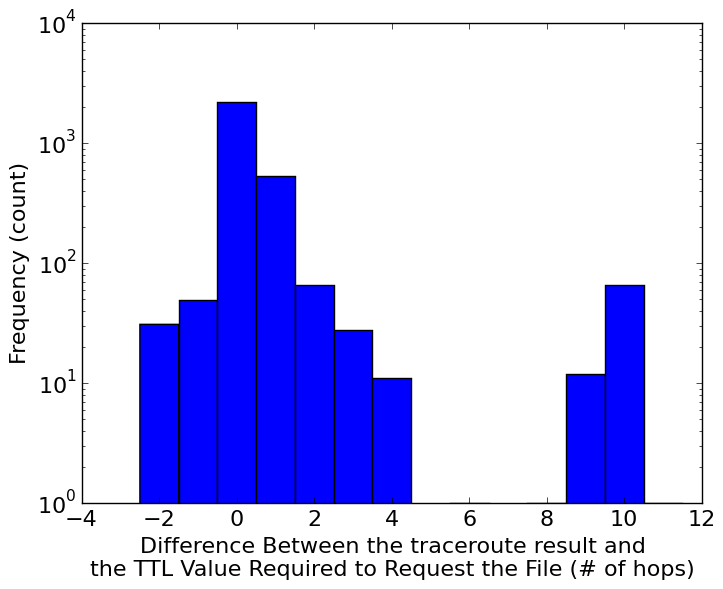
\includegraphics[width=\columnwidth]{figures/histhomepages}
	\caption{
		A histogram showing how often a file request succeeded with a TTL value less than the number of hops to the server (as estimated by \texttt{tcptraceroute}~\cite{Toren2006}), when downloading files from URIs scraped by the homepage-only crawler.
		A zero value on the x-axis represents files which were not received until the TTL value of the request was set to the result of the \texttt{tcptraceroute}.
		Larger values on the x-axis represent files which were received when the TTL value of the request was less than the result of the \texttt{tcptraceroute}.
		Negative values represent files which were not received until the TTL value of the request was set to be greater than the result of the \texttt{tcptraceroute}.
		Files which were not received even when the request was sent with a TTL value 3 greater than the \texttt{tcptraceroute} result are not shown.
	}
	\label{fig_histhomepages}
\end{figure}

The probe was also successfully run on the partial list of 0.9 million URIs generated by the full-site crawler described in \autoref{full-crawler}.
Again erroneous distance estimates were corrected by re-running \texttt{tcptraceroute} in cases where it failed originally.
In addition, a quick scan of the data shows that all of the scripts for which the difference between the \texttt{tcptraceroute} result and the TTL value required for download was greater than 4 are hosted on one of the three domains:
\begin{itemize}\addtolength{\itemsep}{-.35\baselineskip}
	\item \texttt{ir.ebaystatic.com},
	\item \texttt{js4.eastmoney.com}, or
	\item \texttt{www.lady8844.com}.
\end{itemize}
The \texttt{tcptraceroute} results recorded by the probe script for these domains was, respectively, 20, 26, and 24.
However, another run of \texttt{tcptraceroute} run on the same system gives results of 16, 21, and 22 on August 24\textsuperscript{th}.
A histogram of the differences between the \texttt{tcptraceroute} result for the serving domain and the minimum TTL value required to obtain each file, and incorporating all of the corrections above, is shown in Figure~\ref{fig_histmemfail}.
\begin{figure}
	\includegraphics[width=\columnwidth]{figures/histmemfail}
	\caption{
		A histogram showing how often a file request succeeded with a TTL value less than the number of hops to the server (as estimated by \texttt{tcptraceroute}, when downloading files from URIs scraped by the full-site crawler prior to failure in DFO mode.
	}
	\label{fig_histmemfail}
\end{figure}